\documentclass{beamer}
\usepackage{amsfonts,amsmath,oldgerm}
\usetheme{sintef}
\usepackage{xeCJK}
% Lingua del testo
\usepackage[english,italian]{babel}

\newcommand{\testcolor}[1]{\colorbox{#1}{\textcolor{#1}{test}}~\texttt{#1}}

\definecolor{newgreen}{rgb}{0.0, 0.5, 0.0}
\definecolor{newred}{rgb}{0.8, 0.0, 0.0}
 
\usefonttheme[onlymath]{serif}

\titlebackground*{assets/background}

\newcommand{\hrefcol}[2]{\textcolor{cyan}{\href{#1}{#2}}}

\title{System call filtering for container security}
\course{ICT Risk Assessment Lecture Exam\\}
\author{Student: Emiliano Sescu\\
Professor: Fabrizio Baiardi}
%\IDnumber{1234567}
\date{12/02/2024}

\begin{document}
\maketitle

\section{Introduction}


\begin{frame}{Containers Vs Virtual Machines}

\begin{columns}
\begin{column}{0.45\textwidth}
\textbf{Linux containers} are primarily used for running large-scale microservice based applications in a cloud environment. 
\vspace{0.35cm}

In contrast to traditional \emph{Virtual Machines}, containers provide a way to virtualize an OS so that multiple workloads can run on a single OS kernel. 
\vspace{0.01cm}

This makes containers very efficient and scalable, but could also endanger the security of the OS kernel.
\end{column}
\begin{column}{0.55\textwidth}
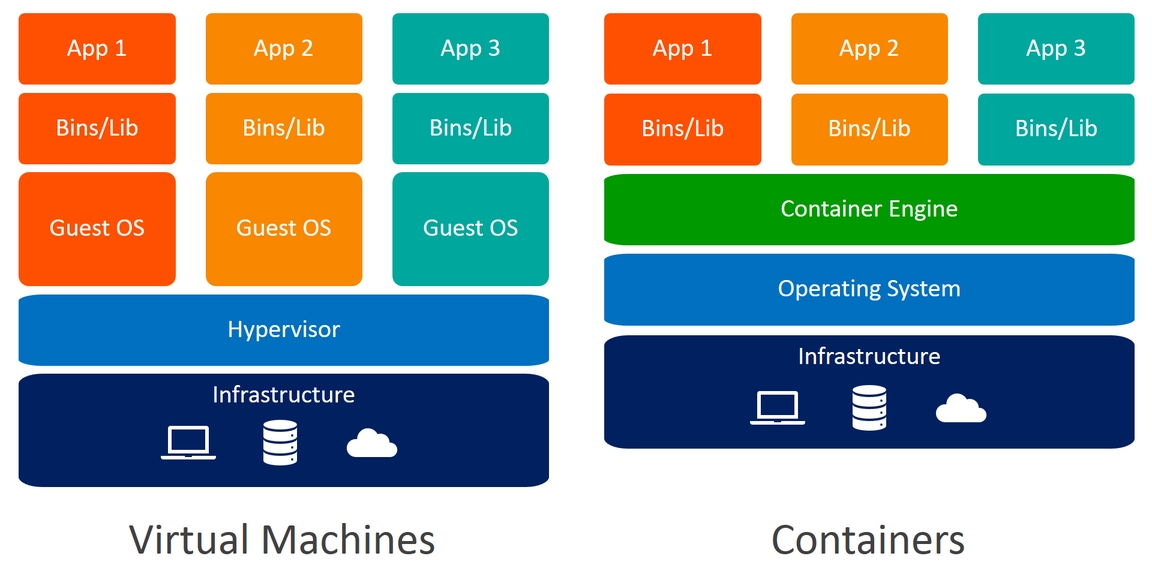
\includegraphics[width=\textwidth]
{assets/containers-vs-virtual-machines}
\end{column}
\end{columns}
\end{frame}

\begin{frame}{Linux kernel mechanisms}

\begin{columns}
\begin{column}{0.45\textwidth}
Despite the use of strict software isolation mechanisms provided by the OS, such as \emph{namespaces}, \emph{cgroups} and \emph{capabilities}, a malicious tenant can leverage kernel vulnerabilities to bypass them.
\vspace{0.35cm}

\textbf{Seccomp} (Secure computing) is a sandbox tool in the Linux kernel to restrict a process from invoking certain system calls.
\end{column}
\begin{column}{0.55\textwidth}
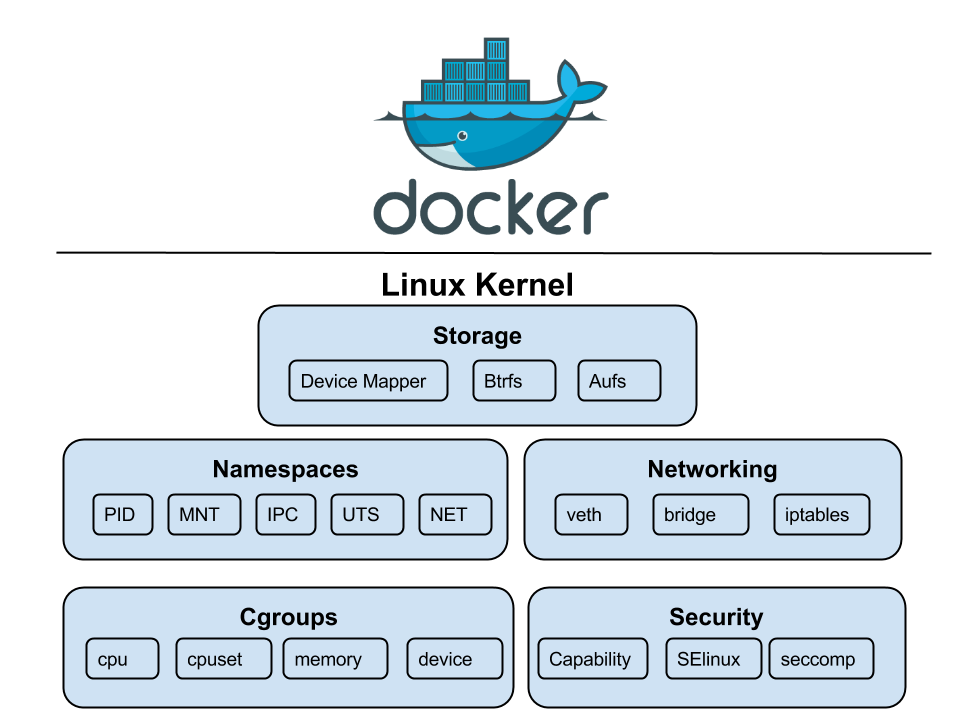
\includegraphics[width=\textwidth]
{assets/linux-kernel}
\end{column}
\end{columns}
\end{frame}


\begin{frame}{Lecture content}
This lecture aims to answer the following two questions:
\begin{itemize}

 \item How it's possible to craft a well-balanced \emph{seccomp profile}?\\

 \item Are there any other techniques to stop adversaries from exploiting kernel vulnerabilities through system call invocations?
\end{itemize}
\vspace{0.3cm}
The tools that will help us to answer those questions are the following ones:

\begin{itemize}

 \item \textbf{Confine} employs an automated technique (using static code analysis) for generating restrictive system call policies for arbitrary container. \\

 \item \textbf{SPEAKER} uses a hybrid container profiling approach that leverages a multi-level static and dynamic analysis methodology to determine the required system calls.\\
 
 \item \textbf{NIMOS} performs a combination of static and dynamic analyses of exploit codes in an automated way and investigated the existence of such commonly occurring system call sequences.
\end{itemize}

\end{frame}

\section{Confine}

\begin{frame}{Design}
By relying on static code analysis, \textbf{Confine} inspects all execution paths of the containerized application and all its dependencies, and identifies the superset of system calls required for the correct operation of the container.

\vspace{0.35cm}
Confine operates in \textbf{three different stage}:
\begin{enumerate}
    \item It first generates a \emph{container-wide system call filter} that is applied to all programs launched in the container. 
    \item Then, it creates an \emph{application-specific system call filter} that removes all system calls needed solely during the initialization phase of the container.
    \item In its final step, Confine further restricts the remaining system calls needed by the main program by \emph{limiting their argument values}.
\end{enumerate}
\end{frame}

\begin{frame}{System calls identification}
The required steps for system calls identification are:
\begin{enumerate}
    \item Identify all applications that may run on the container.
    \item Identify all library functions imported by each application.
    \item Map library functions to system calls.
    \item Extract direct system call invocations from applications and libraries.
    \item Extract hardcoded argument values for identified system calls.
\end{enumerate}
%\hspace*{0.5cm}
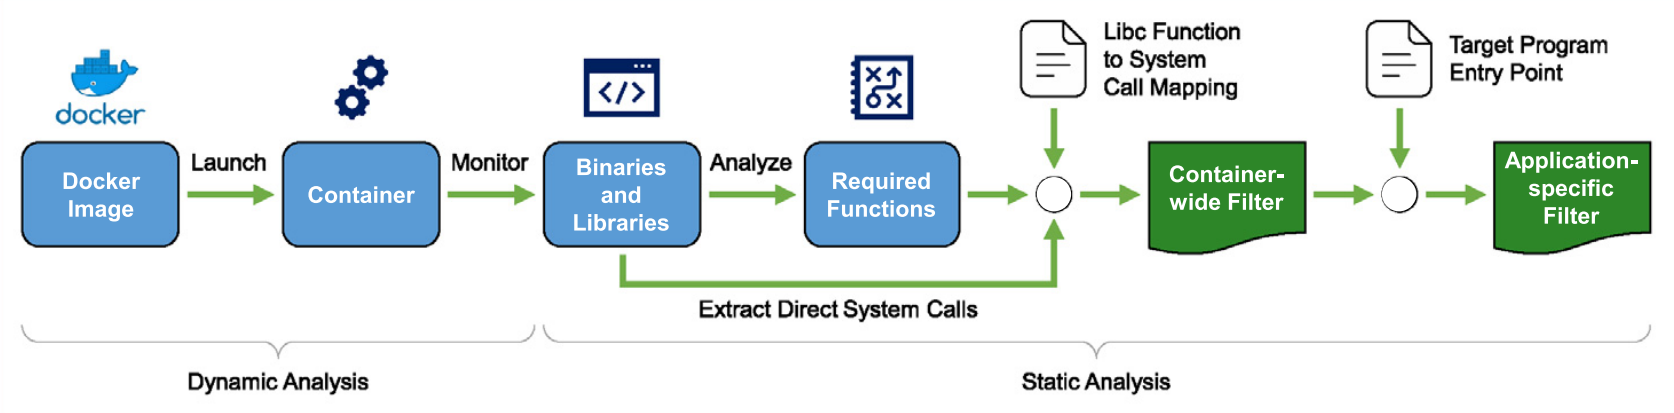
\includegraphics[width=1\textwidth]
{assets/Confine/Confine-design.PNG}
\end{frame}

\begin{frame}{Results: Seccomp profiles of 27 Docker images}
Number of disabled system calls by container-wide (bottom part) and
application-specific (middle part) filtering, and of argument restricted system calls (top part):
\hspace*{1cm}
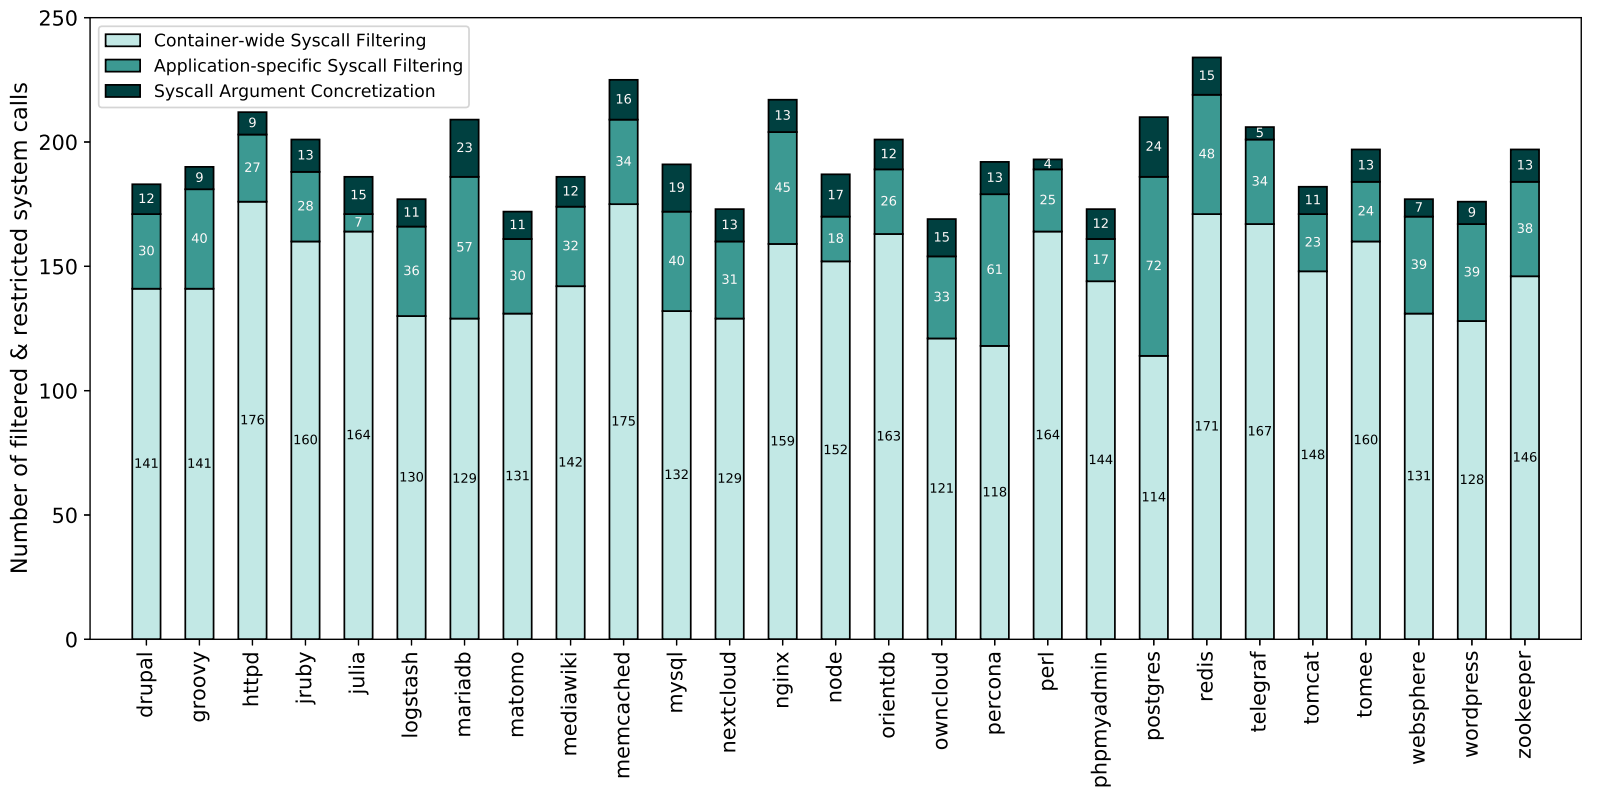
\includegraphics[width=0.8\textwidth]
{assets/Confine/Confine-filter.PNG}
\end{frame}

\begin{frame}{Results: Mitigated CVEs for 27 Docker images}
Given a set of 42 CVEs (extracted from \url{www.cvedetails.com}), it's possible to notice how the addition of \textit{argument concretization} offers a significant improvement:
\hspace*{1cm}
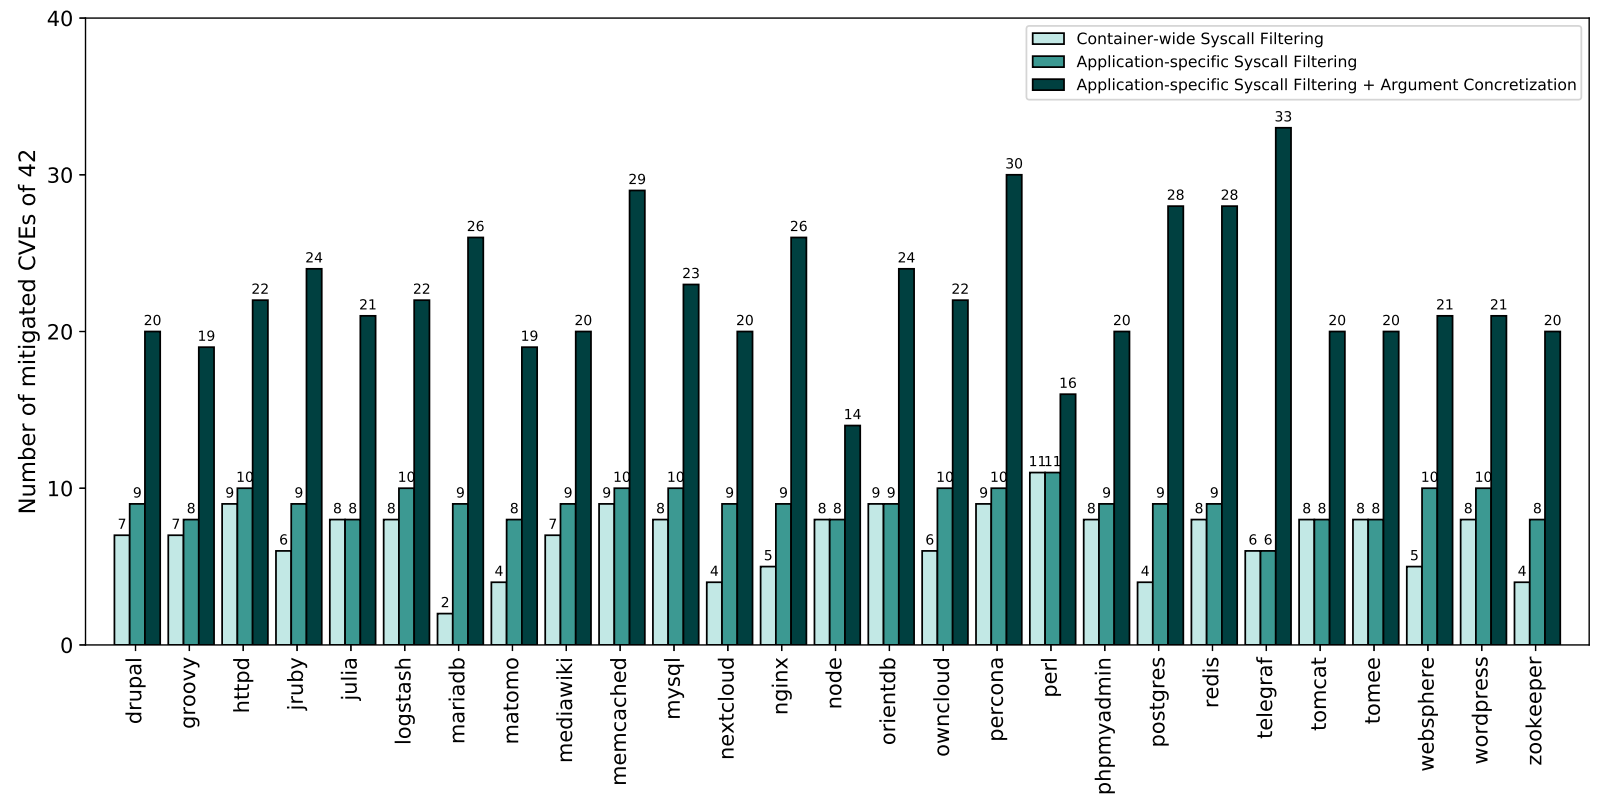
\includegraphics[width=0.8\textwidth]
{assets/Confine/Confine-results.PNG}
\end{frame}

\begin{frame}{Benefits and Drawbacks}
\begin{columns}
\begin{column}{0.5\textwidth}
Benefits:
\begin{itemize}
    \item[\textcolor{newgreen}{\textbullet}] Generate restrictive system call filters and enforce them using a ready-to-use technique
    \item[\textcolor{newgreen}{\textbullet}] Non-intrusive approach
\end{itemize}
Drawbacks:
\begin{itemize}
    \item[\textcolor{newred}{\textbullet}] Only records dynamically loaded libraries during the initial stages of the container execution
    \item[\textcolor{newred}{\textbullet}] Relies on the user to provide informations about the image
\end{itemize}
\end{column}
\begin{column}{0.5\textwidth}
\begin{itemize}
    \item[\textcolor{newred}{\textbullet}] Docker images analyzed by Confine must be compatible with Angr for extracting the CFG of the invoked programs and its libraries
    \item[\textcolor{newred}{\textbullet}] Suffers from overestimating reachable system calls or missing true ones
    \item[\textcolor{newred}{\textbullet}] Confine strives to only restrict flags and constant arguments
    \item[\textcolor{newred}{\textbullet}] Confine proxy program itself requires a limited set of system calls to install the application-specific filter
\end{itemize}
\end{column}
\end{columns}
\end{frame}



\section{SPEAKER}

\begin{frame}{Design}
\textbf{SPEAKER} consists in an hybrid approach to limit the system calls usage: given an application container, a whitelist extracted via \emph{static analysis} is enforced along with a complementary whitelist generated with the \emph{dynamic profiling} of the Docker image.

\vspace{0.2cm}
This method automatically analyzes the container behavior to identify \textbf{three execution phases} (\emph{booting}, \emph{running}, \emph{shutdown}) and  dynamically enforce the corresponding fine-grained system call whitelists. 

\vspace{0.2cm}
The final seccomp profile for each execution phase is determined by both results of the lists obtained with static and dynamic analysis:
\begin{itemize}
    \item If a process invokes a syscall out of the static and dynamic whitelists, it will be killed
    \item If the invoked system call is found only in the static profile, it will be logged for further inspection
    \item If the invoked system call is found within the dynamic profile, it will be normally executed
\end{itemize}
%\hspace*{1.4cm}
%\includegraphics[width=0.8\textwidth]
%{assets/Confine/Confine-design.PNG}
\end{frame}

\begin{frame}{Multi-level approach}
\begin{columns}
\begin{column}{0.5\textwidth}
As illustrated in the figure on the right, the implemented multi-level approach consists of two main components: \textbf{static profiling} and \textbf{dynamic profiling}.
%\vspace{0.35cm}
\end{column}
\begin{column}{0.5\textwidth}
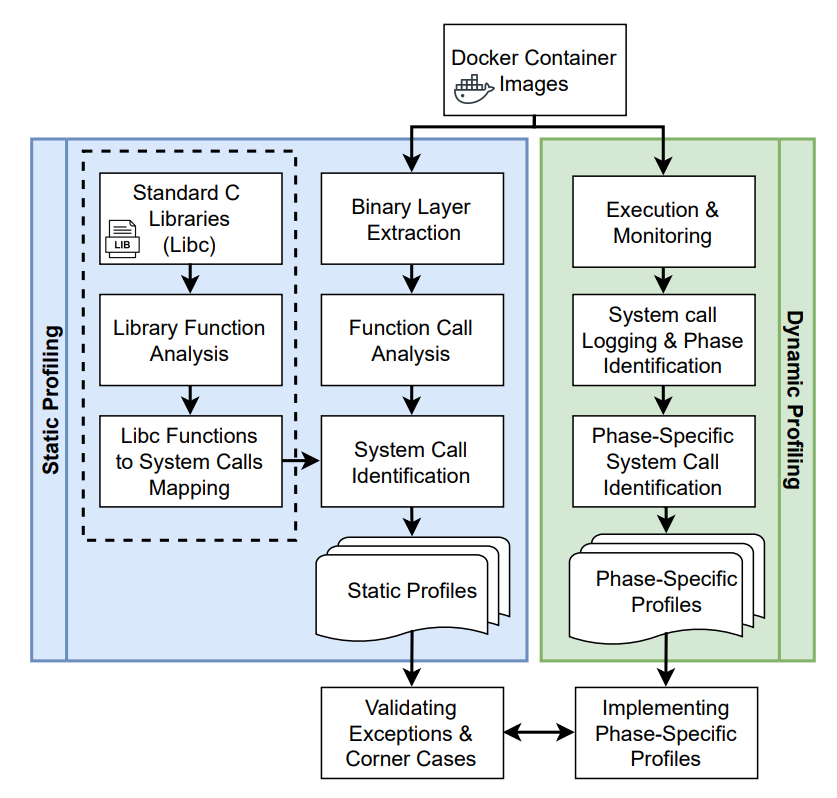
\includegraphics[width=1\textwidth]
{assets/SPEAKER/SPEAKER-design.PNG}
\end{column}
\end{columns}
\end{frame}

\begin{frame}{Results: Static profiling of 150 Docker images}
Comparison with Confine over the required system calls for every image category:
\hspace*{2.3cm}
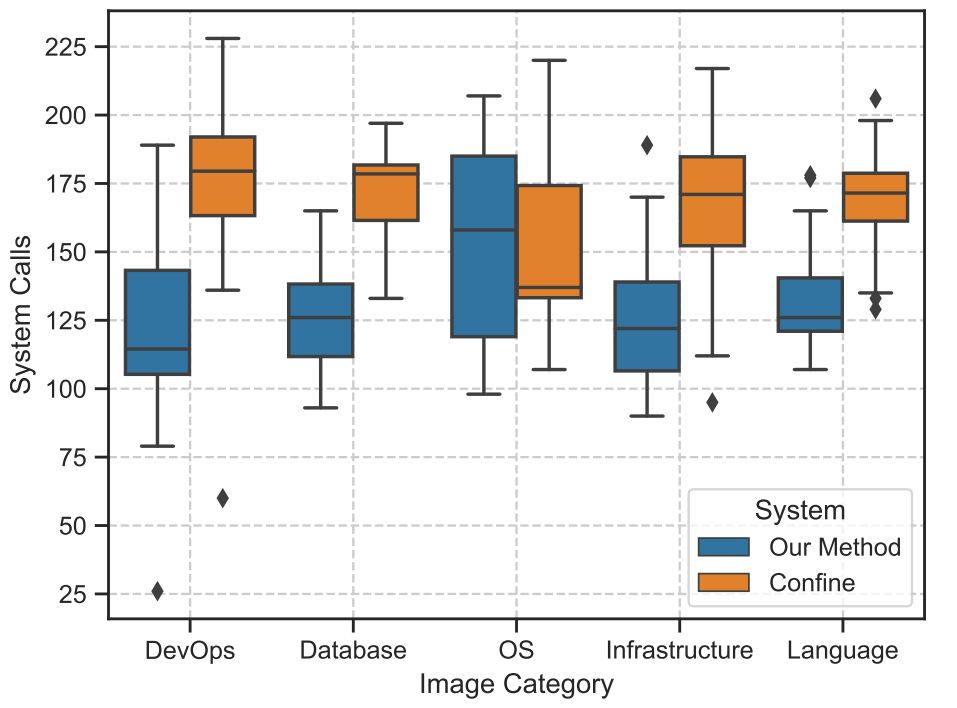
\includegraphics[width=0.65\textwidth]
{assets/SPEAKER/Confine-vs-SPEAKER.PNG}
\end{frame}

\begin{frame}{Experimental results for database and web server containers}
For the vulnerability reduction study, 92 \textit{CVE entry-related} (extracted from \url{cve.mitre.org}) and 21 \textit{high-privileged system calls} were taken into consideration.
\vspace*{0.35cm}
\begin{columns}
\begin{column}{0.5\textwidth}
Number of identified system calls during booting, running, and shutdown execution phase:
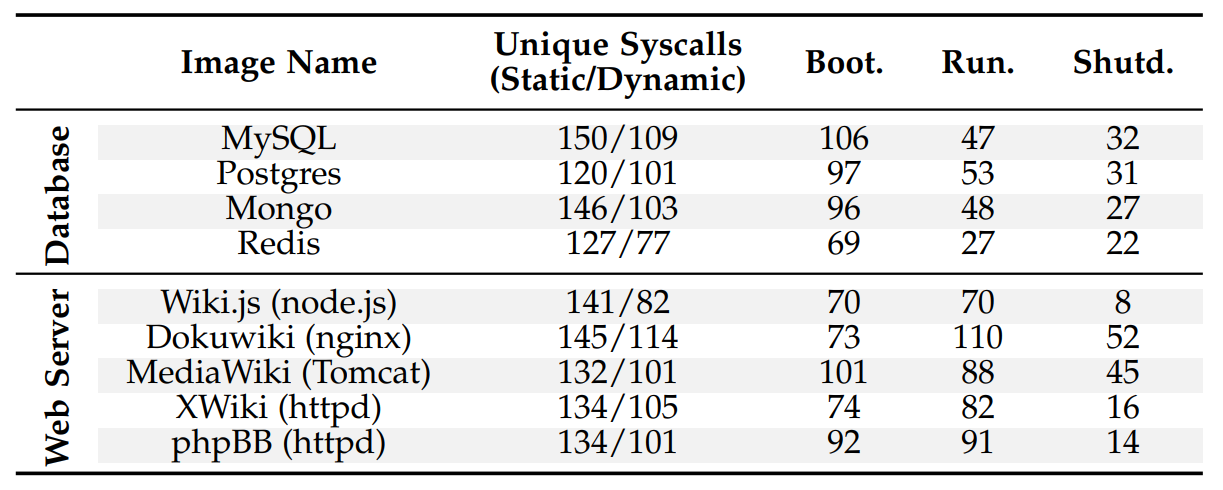
\includegraphics[width=1\textwidth]
{assets/SPEAKER/SPEAKER-results.PNG}\centering
\end{column}\vspace*{0.55cm}
\begin{column}{0.5\textwidth}
Number of required/removed vulnerable syscalls related to CVEs/high-privileged functionalities:
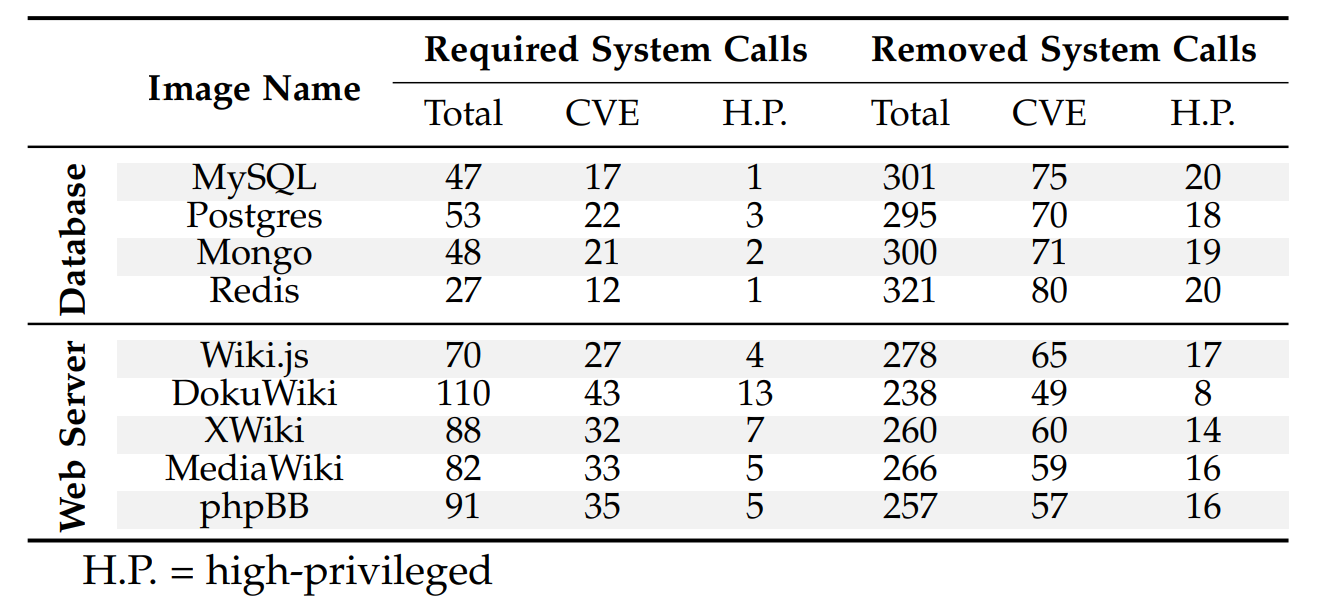
\includegraphics[width=1\textwidth]
{assets/SPEAKER/SPEAKER-security.PNG}\centering
\vspace*{-0.4cm}
\end{column}
\end{columns}
\end{frame}

\begin{frame}{Performance overhead for database and web server containers}
\hspace*{0.65cm}
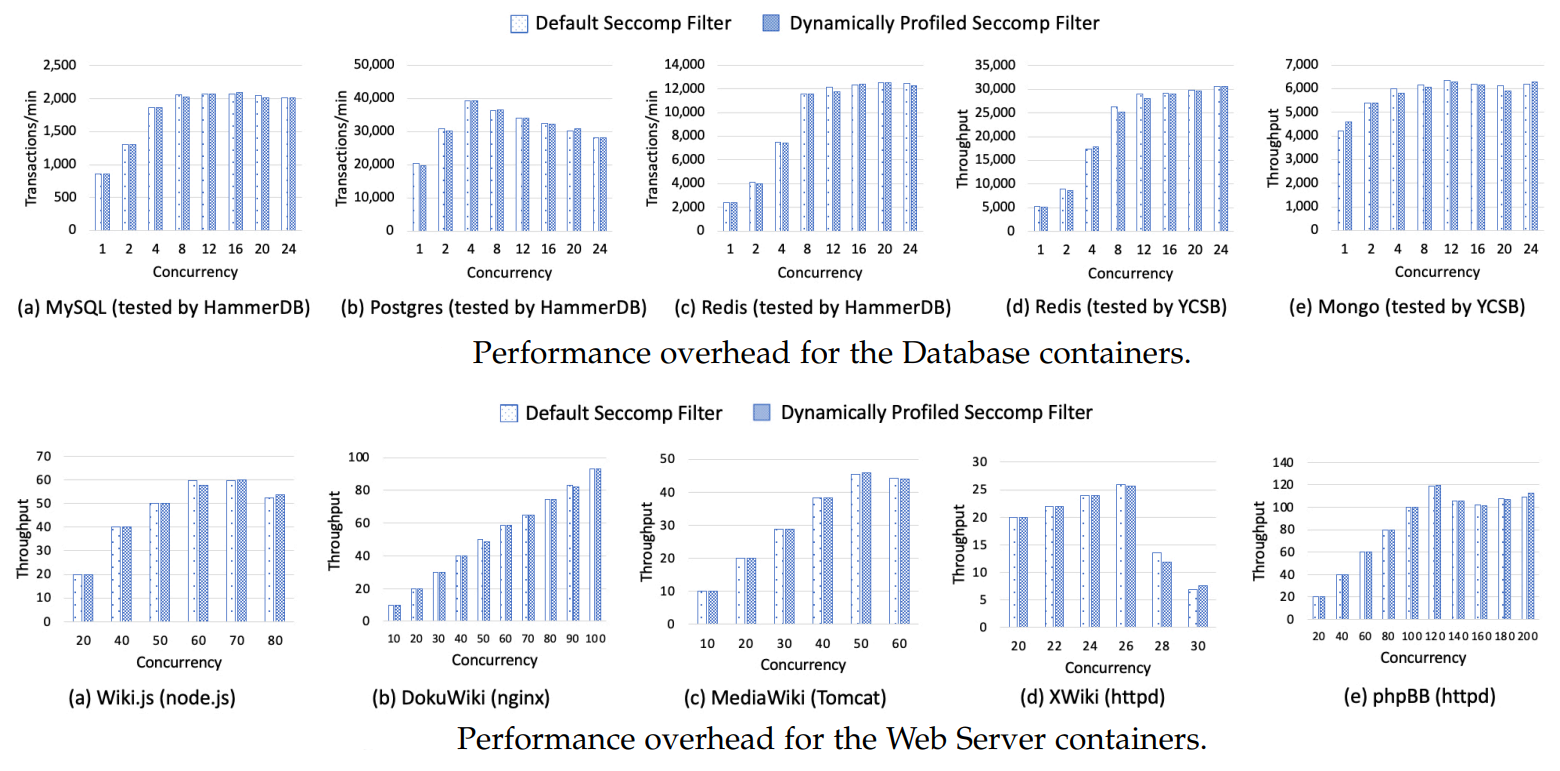
\includegraphics[width=0.9\textwidth]
{assets/SPEAKER/SPEAKER-performance.PNG}
\end{frame}

\begin{frame}{Benefits and Drawbacks}
\begin{columns}
\begin{column}{0.5\textwidth}
Benefits:
\begin{itemize}
    \item[\textcolor{newgreen}{\textbullet}] Better static profiling technique
    \item[\textcolor{newgreen}{\textbullet}] Non-intrusive approach
    \item[\textcolor{newgreen}{\textbullet}] Dynamic profiling reduce overestimation of required system calls of the containerized apps that are based on interpreters
    \item[\textcolor{newgreen}{\textbullet}] Leverages Dynamic profiling with a reasonable performance overhead
\end{itemize}
\end{column}
\begin{column}{0.5\textwidth}
Drawbacks:
\begin{itemize}
    \item[\textcolor{newred}{\textbullet}] Dynamic profiling requires testing tools and benchmarking datasets
    \item[\textcolor{newred}{\textbullet}] Limitations of static analysis
    \item[\textcolor{newred}{\textbullet}] Sanity checking on the parameters of system calls is not performed
    \item[\textcolor{newred}{\textbullet}] The system calls required only for the container initialization are not removed from the static profile
    \item[\textcolor{newred}{\textbullet}] The timing-based method used for phase identification requires some extra system calls
    \item[\textcolor{newred}{\textbullet}] A SPEAKER process runs outside the containers to enforce dynamic profiles
\end{itemize}
\end{column}
\end{columns}
\end{frame}

\section{NIMOS}

\begin{frame}{Design}
\textbf{NIMOS} performs a combination of static and dynamic analyses of exploit codes in an automated way and investigated the existence of such \emph{commonly occurring system call sequence}.
\vspace{0.2cm}

Common system call sequence patterns across the different exploits are then \emph{mined}, and their effectiveness for sequence-based filtering is analyzed.
\end{frame}

\begin{frame}{Design for sequence extraction}
Architecture of NIMOS and processes for system call \textit{sequence extraction and analysis}:
\hspace*{0.9cm}\vspace{0.2cm}
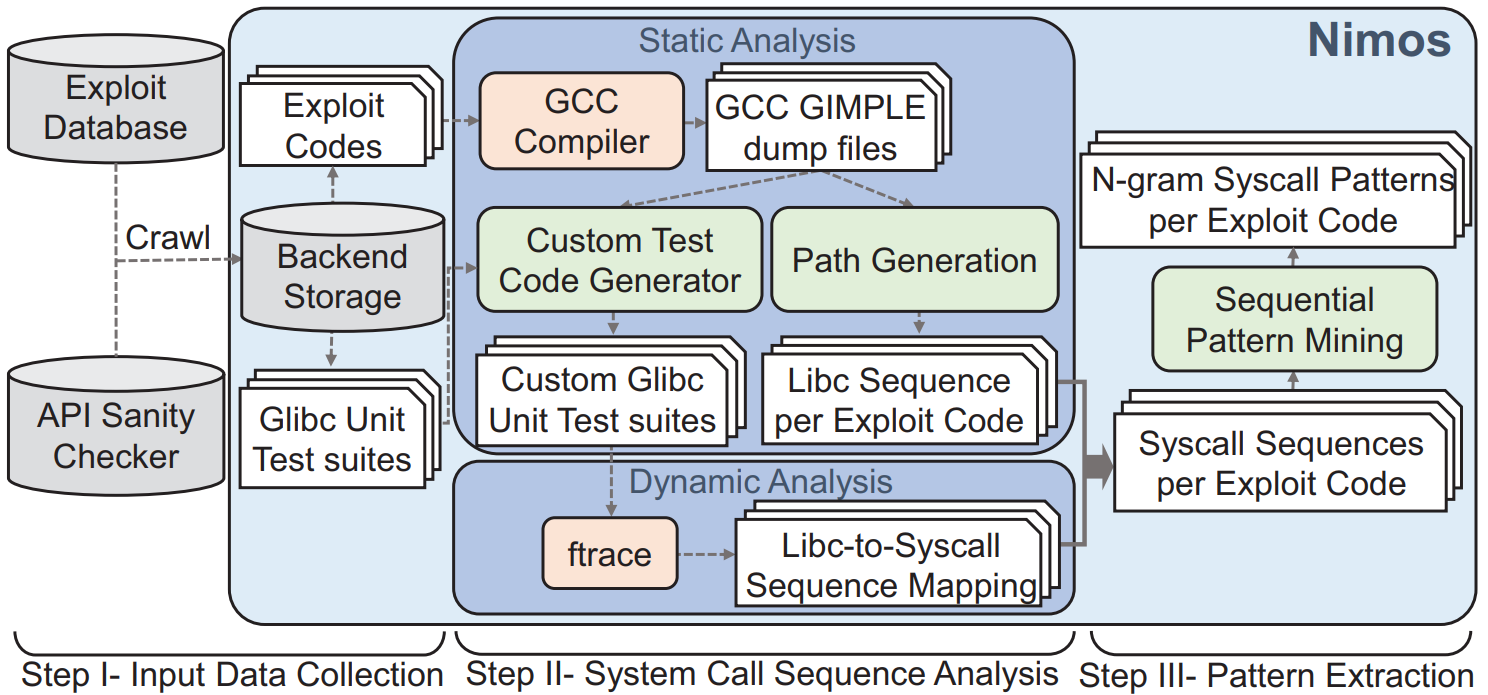
\includegraphics[width=0.87\textwidth]
{assets/NIMOS/NIMOS-design.PNG}
\end{frame}

\begin{frame}{Results: Syscall Sequence Patterns across Exploits}
471 \textit{system call sequence patterns} were found across 106 exploit codes (extracted from \url{www.exploit-db.com}). 
\vspace{0.35cm}

The figure below shows a distribution of the number of patterns discovered and the number of exploit codes matched, for each pattern length:
\hspace*{0.9cm}\vspace{0.2cm}
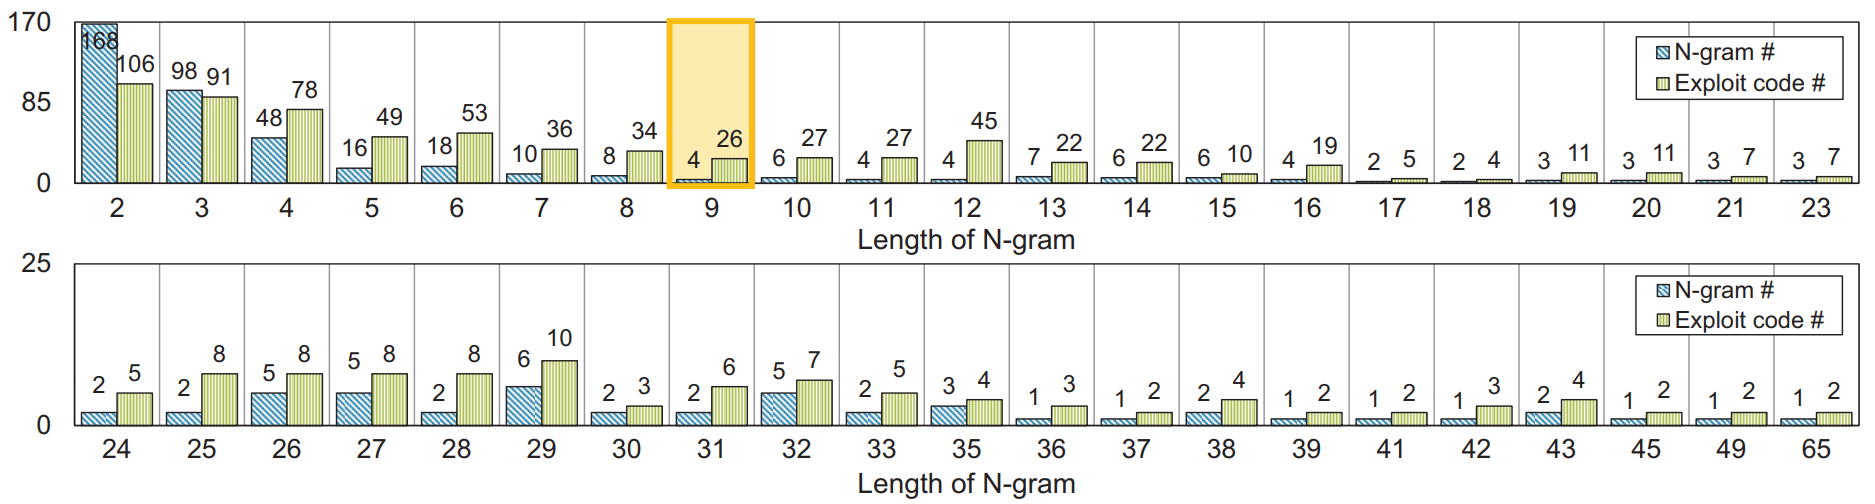
\includegraphics[width=1\textwidth]
{assets/NIMOS/NIMOS-N-grams.PNG}
\end{frame}

\begin{frame}{Results: Syscall Sequence Patterns across Exploits}
Cumulative exploit coverage as N-grams is collectively used in the range of length 65 and downward:
\hspace*{1.5cm}
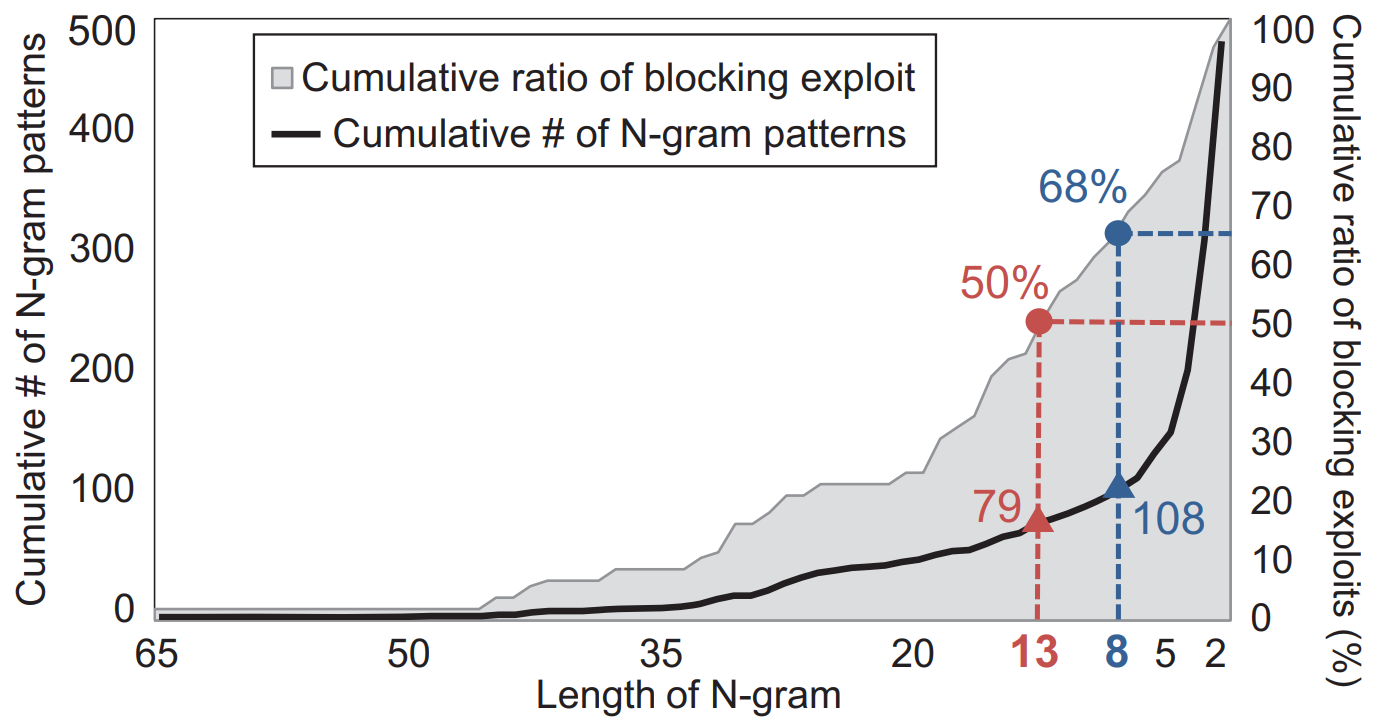
\includegraphics[width=0.8\textwidth]
{assets/NIMOS/NIMOS-blocking-ratio.PNG}
\end{frame}

\begin{frame}{Analysis of Benign Syscall Sequence}
Given a set of 15 popular applications, the figure below shows the number of N-gram syscall sequence patterns from exploit codes found in application traces and the proportion of applications having N-gram syscall sequence patterns from exploit codes:
\hspace*{2cm}
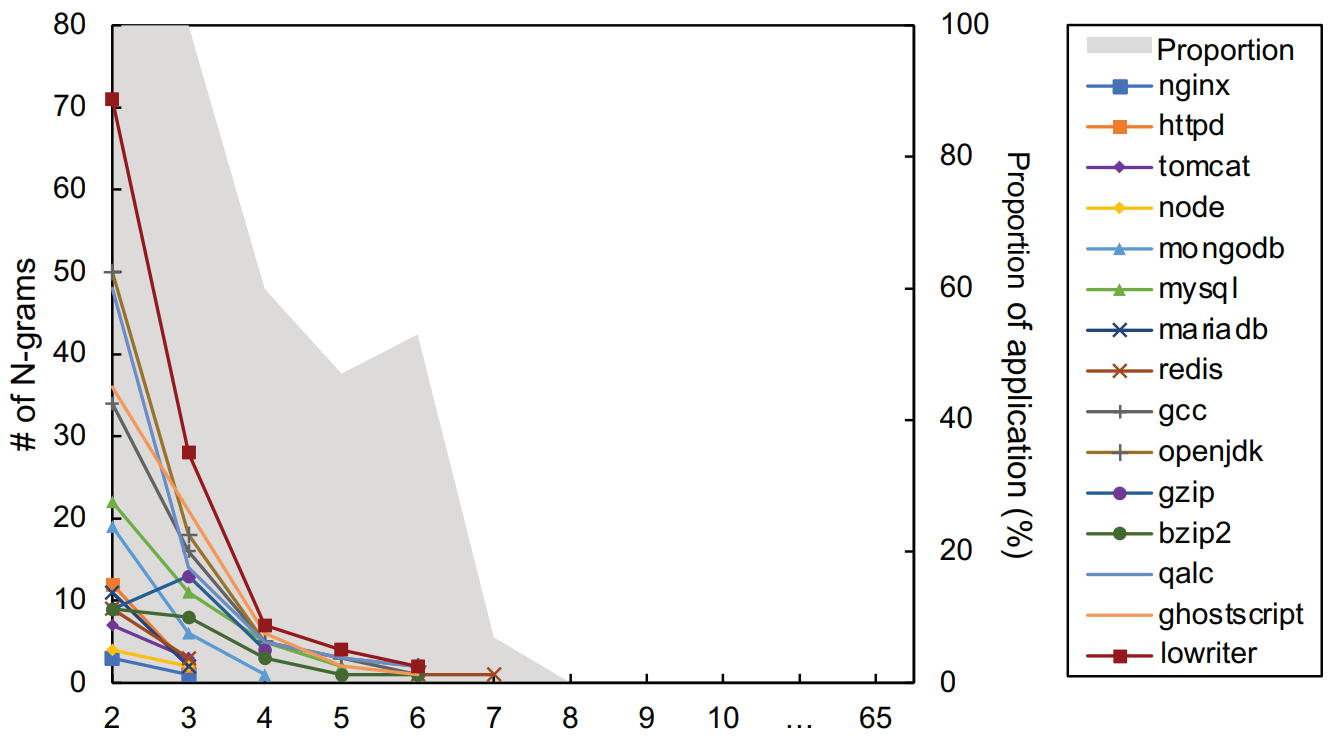
\includegraphics[width=0.7\textwidth]
{assets/NIMOS/NIMOS-benign.PNG}
\end{frame}

\begin{frame}{Container Security Enhancement with Syscall Sequence}
The second column of the table (Ex.) below shows the number of exploit codes that cannot be mitigated even if Confine's seccomp profiles are in place. The third column (Mitigable Ex.) shows how many of the exploits in the second column can be mitigated using syscall sequence patterns. %It shows that, overall, 86.4\% of the exploit codes that could not be mitigated by Confine’s seccomp profile are block-able by our approach.
\hspace*{0.6cm}
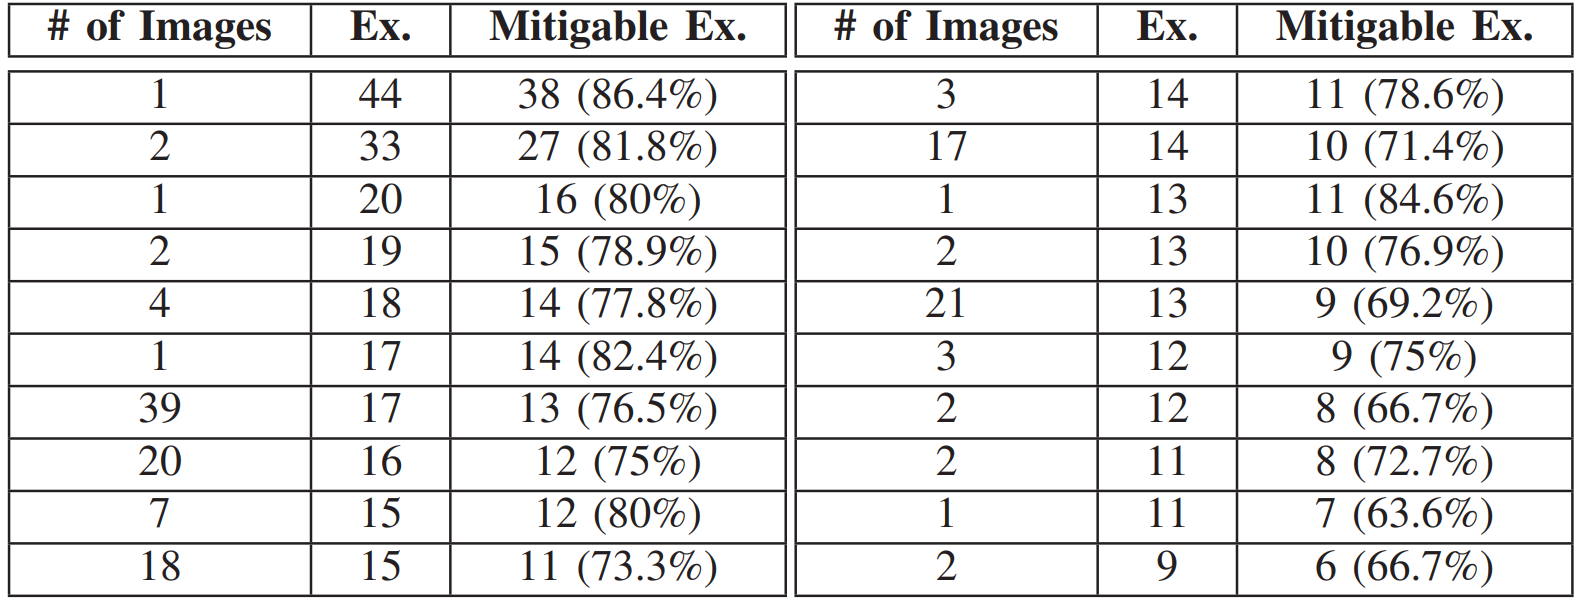
\includegraphics[width=0.9\textwidth]
{assets/NIMOS/NIMOS-vs-Confine.PNG}
\end{frame}

\begin{frame}{Benefits and Drawbacks}
\begin{columns}
\begin{column}{0.5\textwidth}
Benefits:
\begin{itemize}
    \item[\textcolor{newgreen}{\textbullet}] It is possible to pair NIMOS with other tools that enchance seccomp security profile of the container
    \item[\textcolor{newgreen}{\textbullet}] Good results for attacks that can still be performed with non-filtrable system calls
\end{itemize}
\end{column}
\begin{column}{0.5\textwidth}
Drawbacks:
\begin{itemize}
    \item[\textcolor{newred}{\textbullet}] Extending the implementation with an algorithm to enable online tracking of system call sequences using seccomp is a challenging problem yet to be solved
    \item[\textcolor{newred}{\textbullet}] The impact on the performance of these algorithms in a container environment is not yet known
    \item[\textcolor{newred}{\textbullet}] Challenges of mimicry attacks%: an attacker can add arbitrary system calls to the attack sequence or replace some with equivalent ones
\end{itemize}
\end{column}
\end{columns}
\end{frame}

\backmatter

\end{document}
